\documentclass[10pt,a4paper]{article}
\usepackage[margin=23mm]{geometry}
\usepackage[T1]{fontenc}
\usepackage[utf8]{inputenc}
\usepackage{lmodern,microtype,amsmath,amssymb,graphicx,booktabs}
\usepackage[font=small,labelfont=bf]{caption}
\usepackage[numbers,sort&compress]{natbib}
\usepackage[colorlinks=true,allcolors=blue]{hyperref}
\hypersetup{pdftitle={Assessing stereo-microscope calibration through depth and apparent-strain consistency},pdfauthor={Jean-Francois Witz},pdfsubject={Manuscript draft and reproducible calibration assessment}}
\usepackage{fancyhdr}
\pagestyle{fancy}\fancyhf{}\fancyhead[L]{\small Stereo-microscope calibration for deformation measurements}
\fancyhead[R]{\small Manuscript draft}\fancyfoot[C]{\thepage}
\setlength{\headheight}{14pt}
\setlength{\parskip}{3pt}
\setlength{\parindent}{12pt}
\title{Assessing stereo-microscope calibration through\protect\\ depth and apparent-strain consistency}
\author{Jean-Fran\c{c}ois Witz\\[3pt]
\small Univ. Lille, CNRS, Centrale Lille, UMR 9013 -- LaMcube\\
\small Laboratoire de M\'ecanique, Multiphysique, Multi\'echelle, France}
\date{11 September 2026}
\begin{document}
\maketitle
\begin{abstract}
Stereo-microscope calibration is commonly assessed through image residuals or reconstructed depth, whereas deformation measurements depend on spatial differences of reconstruction errors. This work examines whether these criteria rank calibration models consistently. A finite-plane polynomial ray field is compared with a forward Soloff-type mapping and a direct stereo-to-object polynomial, using identical detected correspondences and nominal target coordinates. Two archived translation series provide 202 stereo pairs spanning 0.70 and 0.08\,mm. Ten planes per series are used for calibration, model order is selected by depth-blocked cross-validation within those planes, and the remaining 91 planes are reserved for evaluation. On the wider sweep, depth discrepancies are similar: 11.61, 11.59 and 12.36\,$\mu$m RMS for the ray, forward and direct models. On the finer sweep, the direct mapping has the smallest depth discrepancy, 5.20\,$\mu$m, while the ray field yields the smallest apparent strain on 1.2\,mm virtual gauges: 185\,$\mu\varepsilon$, compared with 268 and 338\,$\mu\varepsilon$. An additional spatial holdout preserves the depth ranking on the fine sweep. Independent perspective simulations with distortion and coordinate noise provide known-depth and known-strain controls. The results demonstrate a model-ranking reversal between depth and length-change consistency on this dataset. They support evaluating calibration against the intended mechanical observable, while distinguishing rigid-target consistency from independently established measurement accuracy.
\end{abstract}
\noindent\textbf{Keywords:} stereo calibration; digital image correlation; microscopy; ray field; apparent strain.

\section{Introduction}
Stereo digital image correlation (DIC) converts image correspondences into surface coordinates and then into displacement and strain. Calibration errors enter this chain before the mechanical quantities are evaluated. A small image residual is therefore useful but insufficient to describe the performance relevant to a deformation experiment. Likewise, a calibration that reproduces nominal depth well need not preserve distances equally well during rigid-body motion. This distinction becomes relevant when only archived calibration images are available and further physical measurements cannot be acquired.

Microscope stereo vision has a substantial history. Schreier et al.\ demonstrated calibration and deformation measurements using distortion estimation and bundle adjustment, including comparison with strain gauges \cite{schreier2004}. Polynomial forward mappings provide another established route: the Soloff formulation describes image coordinates as functions of object coordinates \cite{soloff1997}, and PYCASO makes this approach available for stereo reconstruction \cite{pycaso2023}. Generic camera models instead associate an image position with a viewing ray. Vision-ray calibration is already established in optical metrology \cite{bothe2010}; flexible central and non-central representations also appear in modern camera calibration \cite{schops2020}. Neither ray-based calibration nor polynomial distortion modelling is introduced here as a new principle.

The issue addressed here is narrower: how should these representations be compared when their intended output is a deformation measurement? Reu's Monte Carlo study explicitly propagated calibration errors to three-dimensional position and motion \cite{reu2013}. The present work adopts this output-oriented view and asks whether depth discrepancy and apparent strain select the same model on existing microscope data. It also examines a finite-plane representation that retains independent camera rays while allowing calibration by linear least squares and reconstruction without iterative inversion.

The contribution is a reproducible comparison with separate calibration and evaluation planes, three operational calibration models, and complementary position, motion and length-change observables. The real-data experiment is a retrospective rigid-target assessment using directly detected fiducials. It does not constitute a complete speckle-DIC validation or an independent measurement of the microscope's optical architecture. The synthetic experiment supplies controlled errors with known coordinates and a prescribed extension, while the archived experiment exposes behaviours absent from the idealised simulation.

\section{Calibration representations}
Let $\mathbf p=(u_L,v_L,u_R,v_R)$ denote a stereo correspondence and $\mathbf X=(X,Y,z)$ its assigned object coordinate. All three models use the same paired observations and the same nominal $\mathbf X$. Object coordinates are expressed in millimetres and image coordinates in pixels. No model receives a refinement of target poses, a model-specific correspondence mask, or additional images.

\subsection{Finite-plane ray field}
For camera $c$, the intersection of a viewing ray with a plane at coordinate $z$ is represented by
\begin{equation}
 \begin{pmatrix}X\\Y\end{pmatrix}
 =\mathbf a_c(u,v)+\zeta\,\mathbf b_c(u,v),
 \qquad \zeta=\frac{z-z_0}{s_z},
 \label{eq:ray}
\end{equation}
where $z_0$ and $s_z$ are the mean and standard deviation of the training depths. Each component of $\mathbf a_c$ and $\mathbf b_c$ is expanded in the complete real Zernike basis through radial order $n$. The image square is mapped inside the unit disk using its centre $(1023.5,1023.5)$ and radius $1023.5\sqrt{2}$ pixels. There are $M=(n+1)(n+2)/2$ modes and $8M$ scalar coefficients for the stereo pair.

For each camera, the design matrix is $[B,\zeta B]$, with $B$ the evaluated Zernike basis, and the two right-hand sides are $X$ and $Y$. Equation~\eqref{eq:ray} thus defines a straight line for every image point, without requiring all lines from a camera to pass through a common centre. Its origin can be fixed unambiguously at $z=z_0$:
\begin{equation}
 \mathbf o_c=(a_{cx},a_{cy},z_0),\qquad
 \mathbf d_c=\frac{(b_{cx}/s_z,b_{cy}/s_z,1)}{\|(b_{cx}/s_z,b_{cy}/s_z,1)\|}.
\end{equation}
The reconstructed point is the midpoint of the closest points on the two camera rays. This is a Euclidean closest-ray construction, not a minimisation of the image residual. Rays parallel to the reference plane are outside this parameterisation, and nearly parallel stereo rays remain ill-conditioned.

The finite reference plane removes the arbitrary choice of an origin along each line. Changing $z_0$ with the corresponding coefficient transformation leaves the lines unchanged. This fixes a representation ambiguity; it does not establish the physical accuracy of the assigned target coordinates. Zernike coefficients here parameterise geometry and are not interpreted as identified optical aberrations.

\subsection{Forward and direct polynomial controls}
The forward model approximates all four image coordinates by polynomials of normalised object coordinates:
\begin{equation}
 \mathbf p=\mathbf F(\widetilde{\mathbf X}),\qquad
 \widehat{\mathbf X}=\arg\min_{\mathbf X}\|\mathbf F(\widetilde{\mathbf X})-\mathbf p\|^2.
 \label{eq:soloff}
\end{equation}
Candidate bases contain all monomials through total degrees 1--4. The Soloff 332 basis is included separately: it contains the 19 cubic monomials except pure $z^3$, giving 76 coefficients for four outputs. Reconstruction uses a vectorised Gauss--Newton procedure initialised by an affine inverse, with damping and backtracking. The comparison is with this explicitly defined Soloff-type fit, not the complete PYCASO workflow with its optional calibration-plane adjustment and acceleration procedures.

The direct model fits
\begin{equation}
 \widehat{\mathbf X}=\mathbf G(\widetilde{\mathbf p}),
 \label{eq:direct}
\end{equation}
using complete polynomials in the four normalised stereo coordinates, with total degree 1--4 and $3\binom{d+4}{4}$ coefficients. Unlike the ray field, this representation requires the joint stereo correspondence and provides no independent viewing ray for either camera. Both direct and ray-based reconstruction avoid a nonlinear solve per point, so computational comparisons must include the direct baseline.

All linear systems use column RMS scaling and singular-value decomposition with relative cutoff $10^{-12}$. Means and scales are obtained from training data alone. The fits are unweighted and unregularised. Their residuals lie in different spaces: object-plane coordinates for Eq.~\eqref{eq:ray}, image coordinates for Eq.~\eqref{eq:soloff}, and object coordinates for Eq.~\eqref{eq:direct}. Consequently, identical observations do not imply an identical noise likelihood. The experiment compares these practical estimators rather than isolating model geometry under a common errors-in-variables formulation.

\section{Data and evaluation protocol}
\subsection{Archived microscope images}
The PYCASO repository supplies two series of 101 stereo pairs, with $2048\times2048$ pixels per image \cite{pycasodata}. The source publication describes two XiQ cameras on a Leica M205C stereo microscope, with an SMC100CC controller, TRA6PPD actuator and M-562F-XYZ support; the backlit target is fabricated by chromium deposition on alumina \cite{pycaso2023}. The archived series span nominal depths 2.65--3.35\,mm in increments of 7\,$\mu$m and 2.96--3.04\,mm in increments of 0.8\,$\mu$m. Depth labels are read from filenames. The ChArUco target contains $16\times12$ squares of nominal side 0.3\,mm, giving 165 internal corners. The board uses the legacy pattern, dictionary DICT\_6X6\_250 and a 0.15\,mm marker side.

The target has visibly different image pose and scale between the two series (Fig.~\ref{fig:data}). Each series is therefore calibrated separately. The fine series is not treated as an independent test of an unchanged instrument calibrated on the wide series. Within each series, assigning fixed target $X,Y$ coordinates and filename $z$ assumes a rigid board translated along the nominal depth direction. Target manufacturing error, stage motion error and departure from this geometry remain possible contributors to the reported discrepancies.

\begin{figure}[tb]
\centering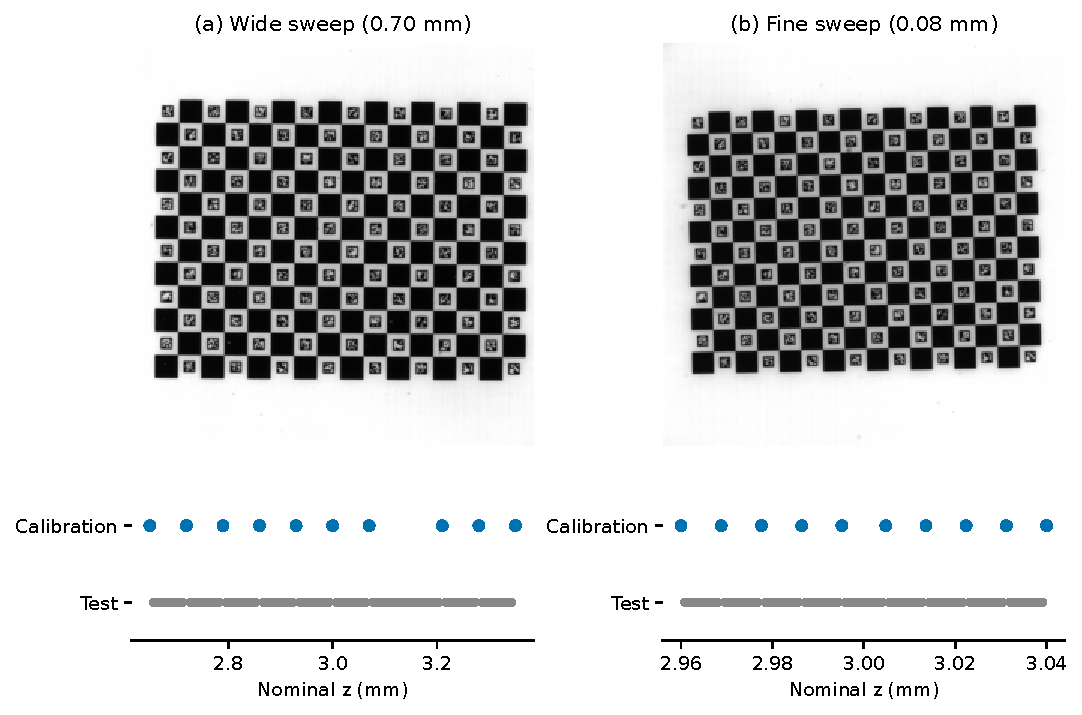
\includegraphics[width=.95\linewidth]{figures/data_protocol.pdf}
\caption{Archived left-camera images at nominal $z=3$\,mm and the plane-level calibration/evaluation split. The two image configurations are fitted independently. All ten calibration planes, including the range endpoints, are excluded from the 91-plane depth evaluation.}
\label{fig:data}
\end{figure}

Corners are detected with OpenCV 4.13.0 ChArUco detection followed by $5\times5$-pixel half-window subpixel refinement, with at most 40 iterations and a $10^{-4}$-pixel stopping threshold. Marker detection uses the parameters retained in the accompanying script. No missing corner is completed and no thin-plate-spline smoothing is applied. Only corners detected in both cameras are retained. The wide series has 61--161 common corners per pair; the fine series has 165 throughout. File hashes and detections are archived with the analysis code \cite{analysiscode}.

\subsection{Selection and held-out evaluation}
In the wide series, calibration uses zero-based plane indices 0, 10, 20, 30, 40, 50, 60, 80, 90 and 100, retaining the ten paired depths of the earlier repository study. Fine-series indices are 0, 11, 22, 33, 44, 56, 67, 78, 89 and 100. These provide respectively 1357 and 1650 paired training corners. The remaining 91 planes contain 13\,444 and 15\,015 evaluation corners.

For each candidate order, one calibration plane is omitted, the model is fitted to the other nine, and depth discrepancy is evaluated on the omitted plane. The selection score is the square root of the mean of these ten plane-wise mean squared discrepancies, with equal weight per plane. The lowest score selects the order within each model family. This criterion is fixed across families and does not use the reported apparent-strain scores. The selected model is then refitted to all ten calibration planes.

This is an interpolation assessment within each sampled depth range. Cross-validation also omits endpoint planes, making some selection folds extrapolations; its score can therefore exceed the final interpolation score. The many corners and planes are not independent repetitions of the experiment. We report descriptive RMS values, without converting their number into a confidence interval on absolute instrument accuracy.

An additional spatial holdout removes alternating target corners from every calibration plane: training uses even $(\mathrm{row}+\mathrm{column})$, while evaluation uses odd parity on the already reserved depth planes. Model orders remain fixed at their primary selected values. This checks spatial interpolation at unused corner identities; it is not a second independent model-selection experiment and does not assess extrapolation beyond the target footprint.

\subsection{Position, motion and virtual-gauge observables}
The pointwise depth score is
\begin{equation}
 E_z=\sqrt{\frac1N\sum_{k=1}^N(\widehat z_k-z_k^{\rm nominal})^2}.
\end{equation}
The reference image is the plane nearest nominal $z=3$\,mm, index 50 in both series. For each evaluation plane, centroid displacement is computed using corner identities common to that plane and the reference. Its depth component is compared with the difference of nominal positions. The reference belongs to the wide calibration set and the fine evaluation set; the fine reference is excluded from motion and gauge averages because comparing a cloud with itself supplies no measurement. There are consequently 91 and 90 evaluated motion states.

Virtual gauges connect corner pairs separated by four squares horizontally or vertically, with nominal reference length 1.2\,mm. For every valid gauge $g$ at plane $t$,
\begin{equation}
 \varepsilon_{g,t}^{\rm app}
 =\frac{\|\widehat{\mathbf X}_{j,t}-\widehat{\mathbf X}_{i,t}\|}
 {\|\widehat{\mathbf X}_{j,0}-\widehat{\mathbf X}_{i,0}\|}-1.
 \label{eq:gauge}
\end{equation}
The denominator is the reconstructed reference length, not its nominal manufactured length. The reported gauge score is the RMS across gauges followed by an equally weighted RMS across evaluation planes. Distances are invariant to rigid translations and rotations; the expected length change for a rigid target is zero. A rigid alignment residual is additionally exported, but no scale adjustment is applied to the clouds.

Apparent gauge strain measures consistency of this complete fiducial/reconstruction chain. It is neither a dense DIC strain map nor an independently calibrated strain uncertainty. Its 1.2\,mm gauge length is essential to interpreting the magnitude: the results should not be transferred directly to a smaller DIC virtual strain gauge.

\subsection{Independent synthetic controls}
An independent distorted-perspective stereo generator places the camera centres at $(\pm12.5,0,0)$\,mm, looking at $(0,0,65)$\,mm, with focal length 25\,600 pixels and principal point $(1023.5,1023.5)$. The same nominal target grid is shifted by $(-2.4,-1.8,62)$\,mm into this world frame. Radial coefficients are $(k_1,k_2,k_3)=(0.8,-2,0.5)$, and tangential coefficients are $(p_1,p_2)=(\pm0.002,-0.003)$. These prescribed values define a numerical control and are not inferred microscope specifications.

Both depth extents are simulated with 101 planes and the ten wide-series calibration indices. Independent Gaussian noise with standard deviation $\sigma=0,0.05,0.2,0.5$ pixels is added to every coordinate of both calibration and test observations. Nonzero noise levels use 20 paired seeds across all models. Fixed cubic models are compared: ray order 3 (80 coefficients), Soloff 332 (76), full cubic Soloff (80), and direct degree 3 (105). This avoids fitting and testing a single shared polynomial generator, while acknowledging that all models approximate the same smooth central-camera control.

For a strain-response check, three unused interior planes, indices 25, 45 and 75, undergo a prescribed $X$ extension of $1000\,\mu\varepsilon$ about the target centre, with zero $Y$ extension. Images are represented by newly projected coordinates, with independent noise in the deformed observations. The same 1.2\,mm horizontal and vertical gauges are reconstructed before and after extension. There are 488 model fits in total, with known-depth and known-strain outputs. These are coordinate-level simulations; image formation, blur, subpixel pattern effects and DIC matching are not simulated.

\section{Results}
\subsection{Controlled depth and strain recovery}
All three implementations recover an affine noiseless stereo geometry to better than $1.5\times10^{-14}$\,mm. A change of ray reference plane leaves the reconstruction unchanged within $1.8\times10^{-15}$\,mm. On eight sampled real correspondences, the vectorised forward-model inverse agrees with a separately evaluated SciPy nonlinear least-squares solve within $10^{-6}$\,mm. These checks address implementation correctness, rather than validation of the physical model.

In the independent perspective control, the noiseless depth RMSE ranges from approximately 0.008 to 0.017\,$\mu$m across the tested models and extents. At $\sigma=0.2$ pixels, the mean depth RMSE is approximately 1.95\,$\mu$m for every model. Figure~\ref{fig:synthetic} shows their near-overlap: there is no substantial ray-field advantage under these conditions. The full cubic forward model and its 332 variant also behave similarly.

\begin{figure}[tb]
\centering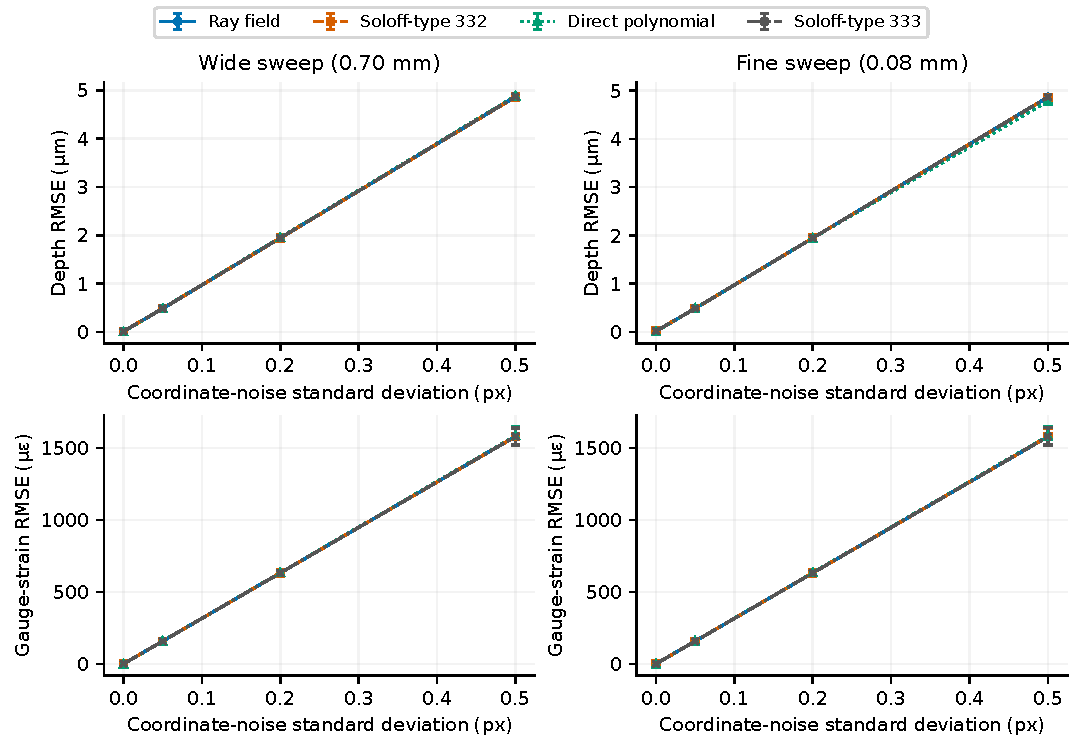
\includegraphics[width=.95\linewidth]{figures/synthetic.pdf}
\caption{Independent distorted-perspective controls. Top: pointwise depth RMSE. Bottom: horizontal-gauge strain RMSE relative to a prescribed $1000\,\mu\varepsilon$ extension. Lines show mean per-run RMSE; error bars show the standard deviation across 20 noise realisations, not a confidence interval for the real instrument. Zero-noise points use one deterministic run. The nearly coincident curves are an experimental result.}
\label{fig:synthetic}
\end{figure}

The horizontal extension is recovered without appreciable attenuation in the noiseless control: all tested model/extent combinations have gauge-strain RMS error below 0.03\,$\mu\varepsilon$. At 0.2-pixel noise, the per-gauge RMS error is approximately 632--634\,$\mu\varepsilon$, while the mean bias over the paired simulations is around $-1\,\mu\varepsilon$. This separates small average bias from substantial local gauge noise. It also shows that low apparent strain is not an inevitable consequence of a ray representation that suppresses all length changes. It does not establish the strain response of the actual calibrated microscope under load.

\subsection{Real-data ranking depends on the observable}
Table~\ref{tab:main} summarises the separately selected models. Wide-series orders are ray 3, forward 4 and direct 4. Fine-series orders are ray 4, forward 332 and direct 1. The fine ray cross-validation scores at orders 3 and 4 differ by only about 0.002\,$\mu$m; the selected degree should not be interpreted as a resolved physical model order.

\begin{table}[tb]
\centering\small
\caption{Primary evaluation on reserved depth planes. $p$ is the coefficient count; $R_{\rm img}$ is training RMS per image coordinate; $E_z$ is pointwise nominal-depth discrepancy; $E_{\Delta z}$ is reference-based centroid-motion discrepancy; $E_\varepsilon$ is apparent gauge strain. All real-data dimensional scores are conditional on nominal target and stage coordinates.}
\label{tab:main}
\begin{tabular}{llrrrrrr}
\toprule
Sweep & Model & Order & $p$ & $R_{\rm img}$ & $E_z$ & $E_{\Delta z}$ & $E_\varepsilon$\\
 & & & & px & $\mu$m & $\mu$m & $\mu\varepsilon$\\
\midrule
\csname @@input\endcsname table_main.tex
\bottomrule
\end{tabular}
\end{table}

On the wide sweep, ray and forward reconstructions have almost identical pointwise depth discrepancies, 11.61 and 11.59\,$\mu$m, despite training image residuals of 0.759 and 0.410 pixels. The direct model gives 12.36\,$\mu$m. Apparent gauge strain is lowest for the forward model, at 383\,$\mu\varepsilon$, compared with 409 for the ray field and 425 for the direct model. The wider sweep therefore does not support a general performance advantage for the ray model.

On the fine sweep, the direct affine mapping gives the smallest pointwise depth discrepancy, 5.20\,$\mu$m, followed by the forward model at 5.89 and the ray field at 9.41\,$\mu$m. The gauge ordering reverses: the ray result is 185\,$\mu\varepsilon$, 31\% below the forward model's 268 and 45\% below the direct model's 338. The ray field thus preserves reconstructed gauge lengths more consistently during this sweep, while recovering nominal depth less well. Figure~\ref{fig:real} displays the depth-dependent structure underlying these aggregate scores.

\begin{figure}[tb]
\centering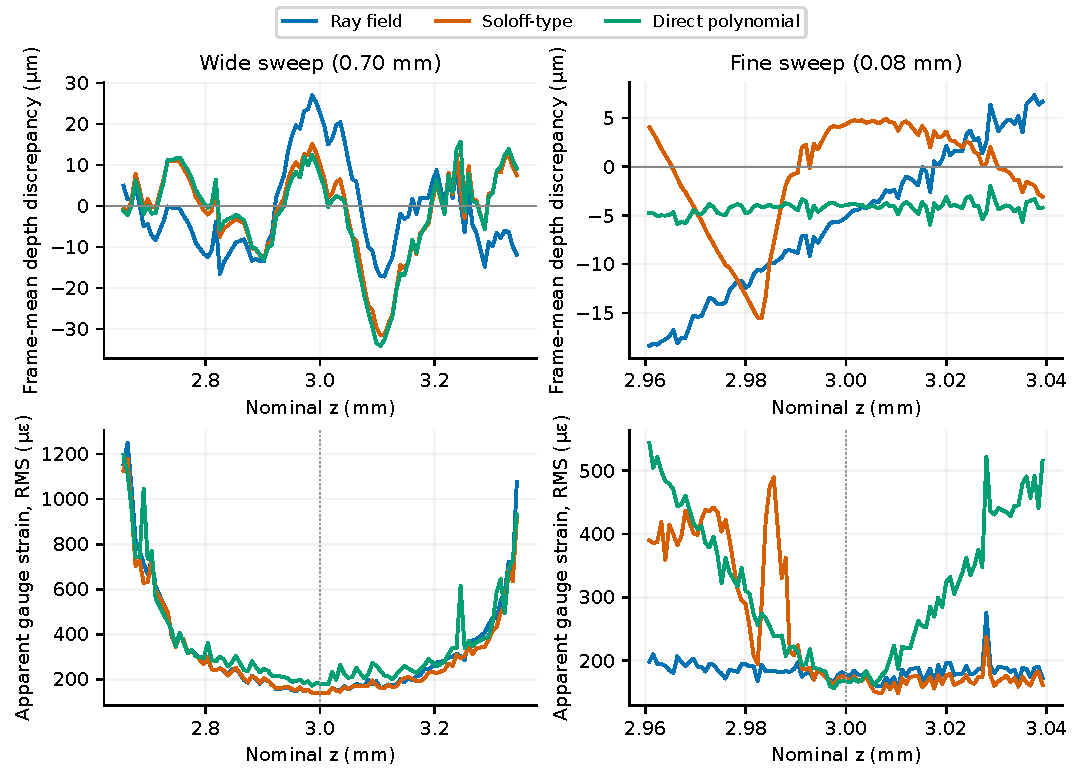
\includegraphics[width=.97\linewidth]{figures/real_observables.pdf}
\caption{Evaluation on real images. Top: frame-mean reconstructed depth minus nominal depth; these signed means differ from the pointwise RMS scores in Table~\ref{tab:main}. Bottom: RMS apparent strain across valid 1.2\,mm gauges at each evaluation plane. The dotted line marks the reference at $z=3$\,mm; its self-comparison is excluded. No model-specific filtering or detrending is applied.}
\label{fig:real}
\end{figure}

Reference-based centroid motion is a distinct observable. On the fine sweep, the direct mapping yields 0.71\,$\mu$m RMS motion discrepancy, compared with 7.58 and 7.70\,$\mu$m for the ray and forward models. A reference-plane error enters all subsequent differences, so a large discrepancy in this quantity need not imply equally large errors between consecutive planes. For the 82 consecutive pairs whose two planes are both reserved, RMS discrepancy in the nominal depth increment is respectively 1.03, 0.98 and 0.77\,$\mu$m for ray, forward and direct models. These values, comparable to the nominal 0.8\,$\mu$m step, do not establish reliable resolution of individual submicrometre motions.

\subsection{Spatial holdout and computational cost}
Table~\ref{tab:additional} reports the additional spatial holdout. The fine-sweep depth ranking is preserved, with discrepancies of 9.26, 5.84 and 4.86\,$\mu$m for the ray, forward and direct models. The wide-sweep ray and forward results remain close to 11.6\,$\mu$m, while the direct result increases to 13.01\,$\mu$m. This supports interpolation consistency at unused target locations within each acquisition, without supplying an independent target or image configuration.

\begin{table}[tb]
\centering\small
\caption{Additional spatial holdout and implementation timing. Spatial training and evaluation use disjoint corner parities as well as disjoint depth planes. Timing instead uses the primary models fitted to all training corners: median of seven evaluations of the same 10\,000 correspondences after one warm-up, with one BLAS thread. Timings describe the supplied Python implementation in a shared x86-64 environment.}
\label{tab:additional}
\begin{tabular}{llrrrr}
\toprule
Sweep & Model & Training points & Test points & Spatial $E_z$ ($\mu$m) & Time (ms)\\
\midrule
\csname @@input\endcsname table_additional.tex
\bottomrule
\end{tabular}
\end{table}

Ray reconstruction takes approximately 5--6\,ms per 10\,000 points in this implementation. The forward polynomial inversion requires approximately 180--318\,ms, and the direct mapping approximately 0.5--5.5\,ms, depending on the selected degree. These are implementation timings rather than universal speed ratios. In particular, the affine direct model is faster than the ray field on the fine sweep. The practical distinction retained by the ray field is independent per-camera geometry with non-iterative triangulation, not exclusive access to fast reconstruction.

\section{Discussion}
\subsection{Why depth and strain rankings can differ}
Depth discrepancy includes spatially common offsets and spatial variation. A length-change measurement instead responds primarily to differences between endpoint errors and to their evolution between images. For a nominally translating gauge with unit direction $\mathbf t_g$ and reference length $L_g$, a first-order approximation gives
\begin{equation}
 \delta\varepsilon_g\simeq\frac{\mathbf t_g^T}{L_g}
 \left[(\mathbf e_{j,t}-\mathbf e_{i,t})-(\mathbf e_{j,0}-\mathbf e_{i,0})\right],
 \label{eq:error}
\end{equation}
where $\mathbf e$ denotes reconstruction error. Spatially common errors cancel to first order; endpoint covariance and changing spatial distortion do not. For nearly in-plane gauges, depth error also need not be the dominant first-order contributor. A criterion based only on $E_z$ cannot therefore determine the strain error.

The fine-sweep result is consistent with this distinction, but the experiment does not identify a unique cause. Ray-line geometry, polynomial approximation, different fitting objectives, target defects and structured corner-localisation errors may all contribute. The near-equivalence of the models in the independent central-camera simulation rules out claiming that the measured ranking reversal is a universal property of generic ray fields. It is a finding about these estimators and these archived image series.

\subsection{Scope of validation and implications for DIC}
The strongest transferable result is the evaluation procedure: reserve acquisition states, compare the same observations, include a direct reconstruction baseline, and report position and length-change consistency separately. DIC users concerned with strain should inspect rigid-motion gauge errors at an appropriate gauge length rather than selecting calibration solely by image residual or depth discrepancy. Conversely, applications dominated by small out-of-plane displacement should retain the direct model as a serious candidate on this dataset.

The evidence has clear boundaries. Stage labels have no accompanying independent uncertainty calibration in this analysis. The target's dimensions, flatness and rigidity are assumed rather than certified. The two series are two acquisitions of a related setup, not a population of microscopes. The spatial holdout interpolates an interlaced grid within a shared field of view. Corner detection replaces speckle matching, and no loaded specimen with independently measured strain is available. The PYCASO publication includes a coin/profilometry comparison, but numerical profilometry data were not found in the inspected repositories and are not reused here as a new independent reference. The simulated noise is independent and Gaussian, whereas real localisation errors can be correlated, anisotropic and dependent on defocus. These limitations prevent interpreting the reported RMS values as an absolute metrological uncertainty budget or a demonstrated improvement in full-field DIC strain accuracy.

Further work that uses the existing material can build on the explicit ray geometry. Examples include propagating an image-coordinate covariance through triangulation and virtual gauges, comparing joint errors-in-variables fits, and evaluating dense correspondence algorithms on the archived images with identical masks. Multi-camera extension is also natural because each camera supplies its own rays. These are potential applications of the representation; none is required to explain the present ranking reversal, and none is claimed as experimentally validated here.

\section{Conclusion}
A short retrospective assessment can extract useful calibration evidence from archived microscope translation images without identifying a detailed optical model. In the examined data, the best model depends on the observable. Ray and forward polynomial models give similar depth discrepancies on the wide sweep. On the fine sweep, a direct affine mapping best follows nominal depth and centroid motion, while the ray field produces the smallest apparent strain on 1.2\,mm gauges. Independent controlled simulations show comparable noise sensitivity across the models rather than a general ray-field advantage. The resulting recommendation is to evaluate calibration in the coordinates of the intended mechanical measurement and to keep rigid-target consistency distinct from independently established accuracy.

\section*{Data and code availability}
The original images are available from PYCASO at commit \texttt{44fbf1a} \cite{pycasodata}. The analysis is based on StereoComplex commit \texttt{ed422d6}; scripts, extracted observations, per-image hashes, all simulation outputs and figure-generation code are provided in \texttt{paper/strain} on the accompanying analysis branch \cite{analysiscode}. Raw images are referenced at their source rather than duplicated. The README gives executable reproduction commands and the exact plane split. No new physical measurement was made for this study.

\bibliographystyle{unsrtnat}
\bibliography{references}
\end{document}
